\documentclass[../main.tex]{subfiles}
\graphicspath{{\subfix{../IMAGES/}}}

\begin{document}
\localtableofcontents
\subsection{Introduction}
Engineering design is a systematic process in which designers generate, evaluate and specify devices, systems or processes whose form and function achieve objectives while satisfying constraints.\\

\begin{itemize}
    \item Mechanical design : the physical principles, the proper functioning, and the production of mechanical systems\\
    \item Industrial design : pattern, color, texture and consumer appeal\\
\end{itemize}

\quad \underline{The Design process :}\\
\begin{enumerate}
    \item Market need : design requirements\\
    \item Concept : determine function structure, seek working principles, evaluate and select concepts\\
    \item Embodiment : develop layout, scale, form, model and analyze assemblies, evaluate and select layouts\\
    \item Detail : analyze components in detail, optimize performance and cost, final choice of material and process\\
    \item Product specification\\
\end{enumerate}

A technical system consists of sub assemblies and components that enable the required task.\\
Decomposition useful for analysing an existing design but challenging for the design process. We need to consider the inputs, flows and outputs of information, energy and materials.\\

When trying to develop a new device, we first need to address a \textbf{solution-neural need statement}. It cannot imply by any mean a characteristic of the product (i.e. we want to develop a product to remove the cork from a bottle of wine, the solution-neural need statement would be : "A device is required to allow access to wine in a corked bottle with convenience, at modest cost, and without contaminating the wine")\\

\quad\underline{Needs statement :}\\
\begin{itemize}
    \item Primary needs (strategic needs)\\
    \item Secondary needs (tactical needs)\\
    \item Tertiary needs (operational needs)\\
    \item Must haves\\
    \item Delighters (latents needs)\\
    \item Linear satisfiers\\
    \item Neutral\\
\end{itemize}

In order to determine the important needs, we use a Kano-Diagram :\\
\begin{figure}
    \centering
    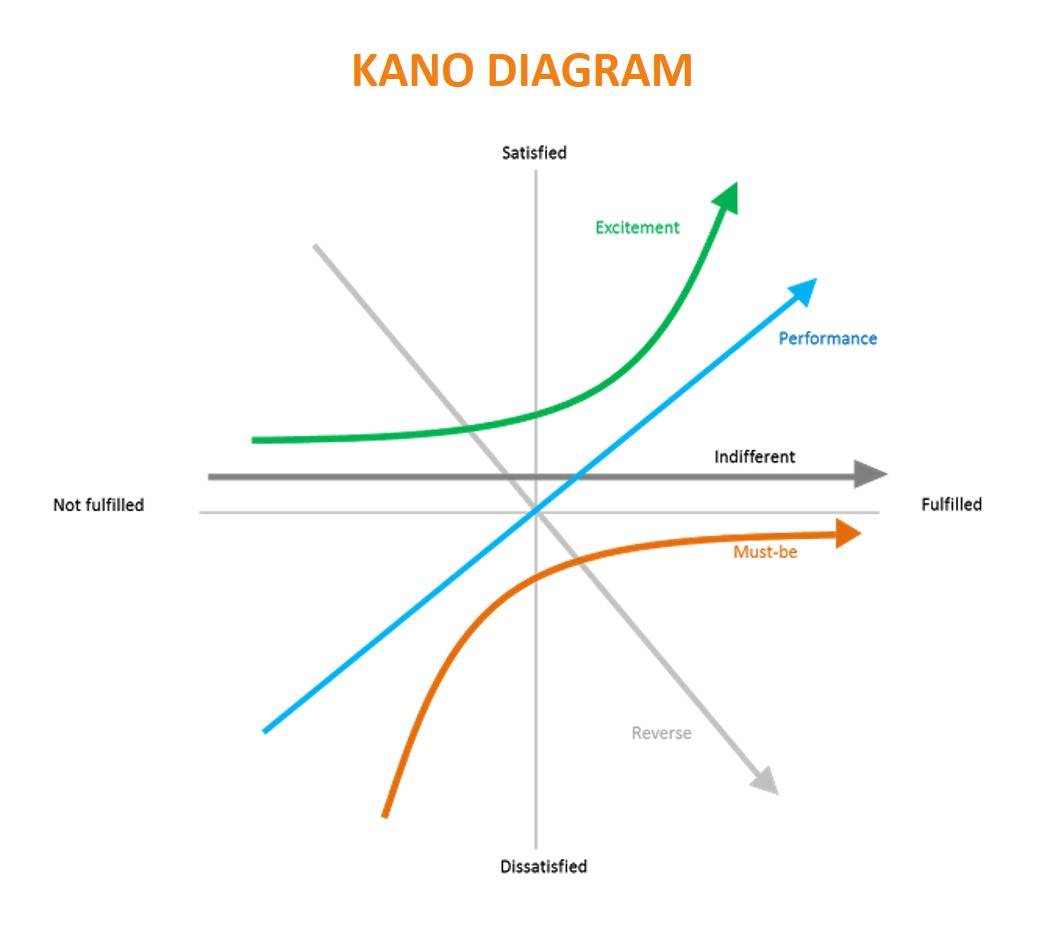
\includegraphics[width=\textwidth]{IMAGES/proddev/Kano+diagram-3561535844.jpeg}
\end{figure}

\subsection{Stages of design}
A product opportunity exists when there is a gap between what is currently on the market and the possibility for new or significantly improved products that result from emerging trends.\\

\quad \underline{The SET factors :}\\
\begin{itemize}
    \item SOCIAL : social and cultural trends and drivers. Reviving historical trends\\
    \item TECHNOLOGY : state of the art and emerging technology. Re-evaluating existing technology\\
    \item ECONOMIC : state of the economy. Shift in focus on where to spend money. Level of disposable income\\
\end{itemize}

Changes in the SET factors product Product Opportunity Gaps (POG). Translate the POG into a new product or a significant modification of an existing product. Combination of new aesthetic or new features. Stemming from new technology. Must match emerging shifts in consumer preference.\\

\textbf{SET Factors in at least 2, if not 3 areas leads to a product opportunity!}\\

\quad \underline{What is a specification ?}\\
Specifications spell out in precise, measurable detail what the product has to do. For simple products, early in the development process, right after identifying customer needs. It consists of a metric and a value. Metrics should be dependent variables and practical. Some needs cannot be translated into quantifiable metrics (subjective needs).\\

\quad \underline{Concept generation :}\\
Concept generation can lead to poor outcomes when \begin{itemize}
    \item consideration of only a few concepts\\
    \item failure to consider  carefully existing solutions\\
\end{itemize}

Five-steps method : \begin{enumerate}
    \item Clarify the problem : decompose into sub problems; functional decomposition\\
    \item Search externally : search for existing solutions/patents\\
    \item Search internally\\
    \item Explore systematically : classification tree (remove less promising branches); combination table\\
    \item Reflect on solution and process\\
\end{enumerate}

The \textbf{concept selection process} is based on two methodologies : \begin{itemize}
    \item concept screening (or Pugh Concept Selection) : to reduce the best concepts/refine further or even generate new concepts\\
    \item concept scoring : select the final solution\\
\end{itemize}

\quad \underline{Concept screening :}
\begin{enumerate}
    \item Prepare selection matrix : choose reference concept\\
    \item Rate the concepts : relative score (+ or -) wrt reference concept\\
    \item Rank the concepts : sum of all the + and -\\
    \item Combine and improve the concepts\\
    \item Select one or more concepts\\
    \item Reflect on results and process\\
\end{enumerate}

\quad \underline{Concept scoring :}\\
Used when increased resolution will better differentiate among competing concepts. It is a more quantitative version of concept screening. We need a scale (from 1 to 5 usually) and weight every selection criteria.\\






\end{document}